\chapter{Estudio sobre el acero F138}\label{C:F138}
\graphicspath{{./figs/04_F138/}}

En este capítulo se estudia la microestructura de un acero inoxidable F138, que es un acero de tipo austenítico, lo que implica que es un material con estructura cristalina de tipo FCC.
El acero se obtuvo comercialmente, y la composición, dada por el fabricante se muestra en la Tabla \ref{tab:F138Comp}.

\begin{table}[!htb]
\centering
\begin{tabular}{|c|c|c|c|c|c|c|c|c|c|c|}
\hline
\rowcolor[HTML]{BBDAFF} 
\textbf{Fe} & \textbf{Cr} & \textbf{Ni} & \textbf{Mo} & \textbf{Mn} & \textbf{Si} & \textbf{Cu} & \textbf{N} & \textbf{C} & \textbf{P} & \textbf{S} \\ \hline
          &    17.33  &   14.31   &   2.79    &   1.79    &  0.30     &   0.09    &   0.079   &  0.015    &   0.022   &   0.002   \\ \hline
\end{tabular}
\caption{Composición del acero inoxidable F138 (\% en peso dado por el fabricante)}
\label{tab:F138Comp}
\end{table}

El acero F138 se caracteriza por tener una elevada resistencia a la corrosión, lo que lo hace útil para aplicaciones biomédicas y en energía nuclear.
Según el estudio realizado por Scheriau et al \cite{Scheriau2011}, cuando se lo somente a deformación plástica severa, tiene dos modos de deformación principales que consisten en maclado mecánico (con maclas de 10-20\,nm de ancho) y bandas de corte submicrométricas que dividen el material en bloques micrométricos de láminas de maclas.
Liu et al. \cite{Liu2010} observaron una respuesta similar en un acero 316L sometido a deformación plástica dinámica, donde la estructura final evolucionó hacia una configuración de granos micrométricos de austenita junto con maclas nanométricas, confiriéndole al material una tensión de fluencia casi cinco veces mayor que aquella correspondiente a la estructura inicial de granos grandes.

El 2.5\% de Mo agregado mejora la resistencia a la corrosión, y al encontrarse en solución sólida contribuye a reducir la movilidad de las dislocaciones \cite{Chowdhury2005}.

El grupo de trabajo al que pertenece el autor de esta tesis tiene antecedentes de trabajo, tanto en muestras laminadas como en muestras deformadas por medio de la técnica de \textit{Deformación de Igual Canal Angular} (ECAE, por sus siglas en inglés)\cite{Devincentis2015PhD,Devincentis2017}, aunque los estudios realizados se concentraron previamente en mediciones de EBSD y en estudios de ancho de pico a través de los métodos de Williamson-Hall y CMWP.
En la Sec. \ref{S:F138Nati} se realiza un repaso de los principales resultados que se tienen sobre este material, mientras que en la Sec. \ref{S:F138LANG} se aplica el método de Langford a muestras de acero F138 laminadas hasta lograr una reducción de la reducción transversal del 70\,\%.

\nomenclature{ECAE}{Equal Angle Angular Extrusion, Deformación de Igual Canal Angular}
\section{Estado del arte en el estudio de la microestructura}\label{S:F138Nati}
En esta sección se presentan los resultados previos obtenidos en el grupo de investigación al que pertenece el autor de esta tesis. Los mismos incluyen mediciones de EBSD y estudios de ancho de pico empleando los métodos de Williamson-Hall y CMWP, y se encuentran publicados en \cite{Devincentis2015PhD,Devincentis2017}.

En la Fig. \ref{fig:F138PF} se encuentran las FP recalculadas a partir de las mediciones de textura realizadas en sincrotrón, donde pueden apreciarse la presencia de la fibra \{110\}\textless uvw\textgreater. 
Las FP de la Fig. \ref{fig:F138PF} provienen de la FDO que se observa en la Fig. \ref{fig:F138ODF}, donde se puede ver más claramente la fibra \{110\}\textless uvw\textgreater, en la sección $\varphi_2 \ = \ 0$\,$^{\circ}$, a lo largo de la coordenada $\Phi \ = \ 45$\,$^{\circ}$.

\begin{figure}[!htb]
  \centering
  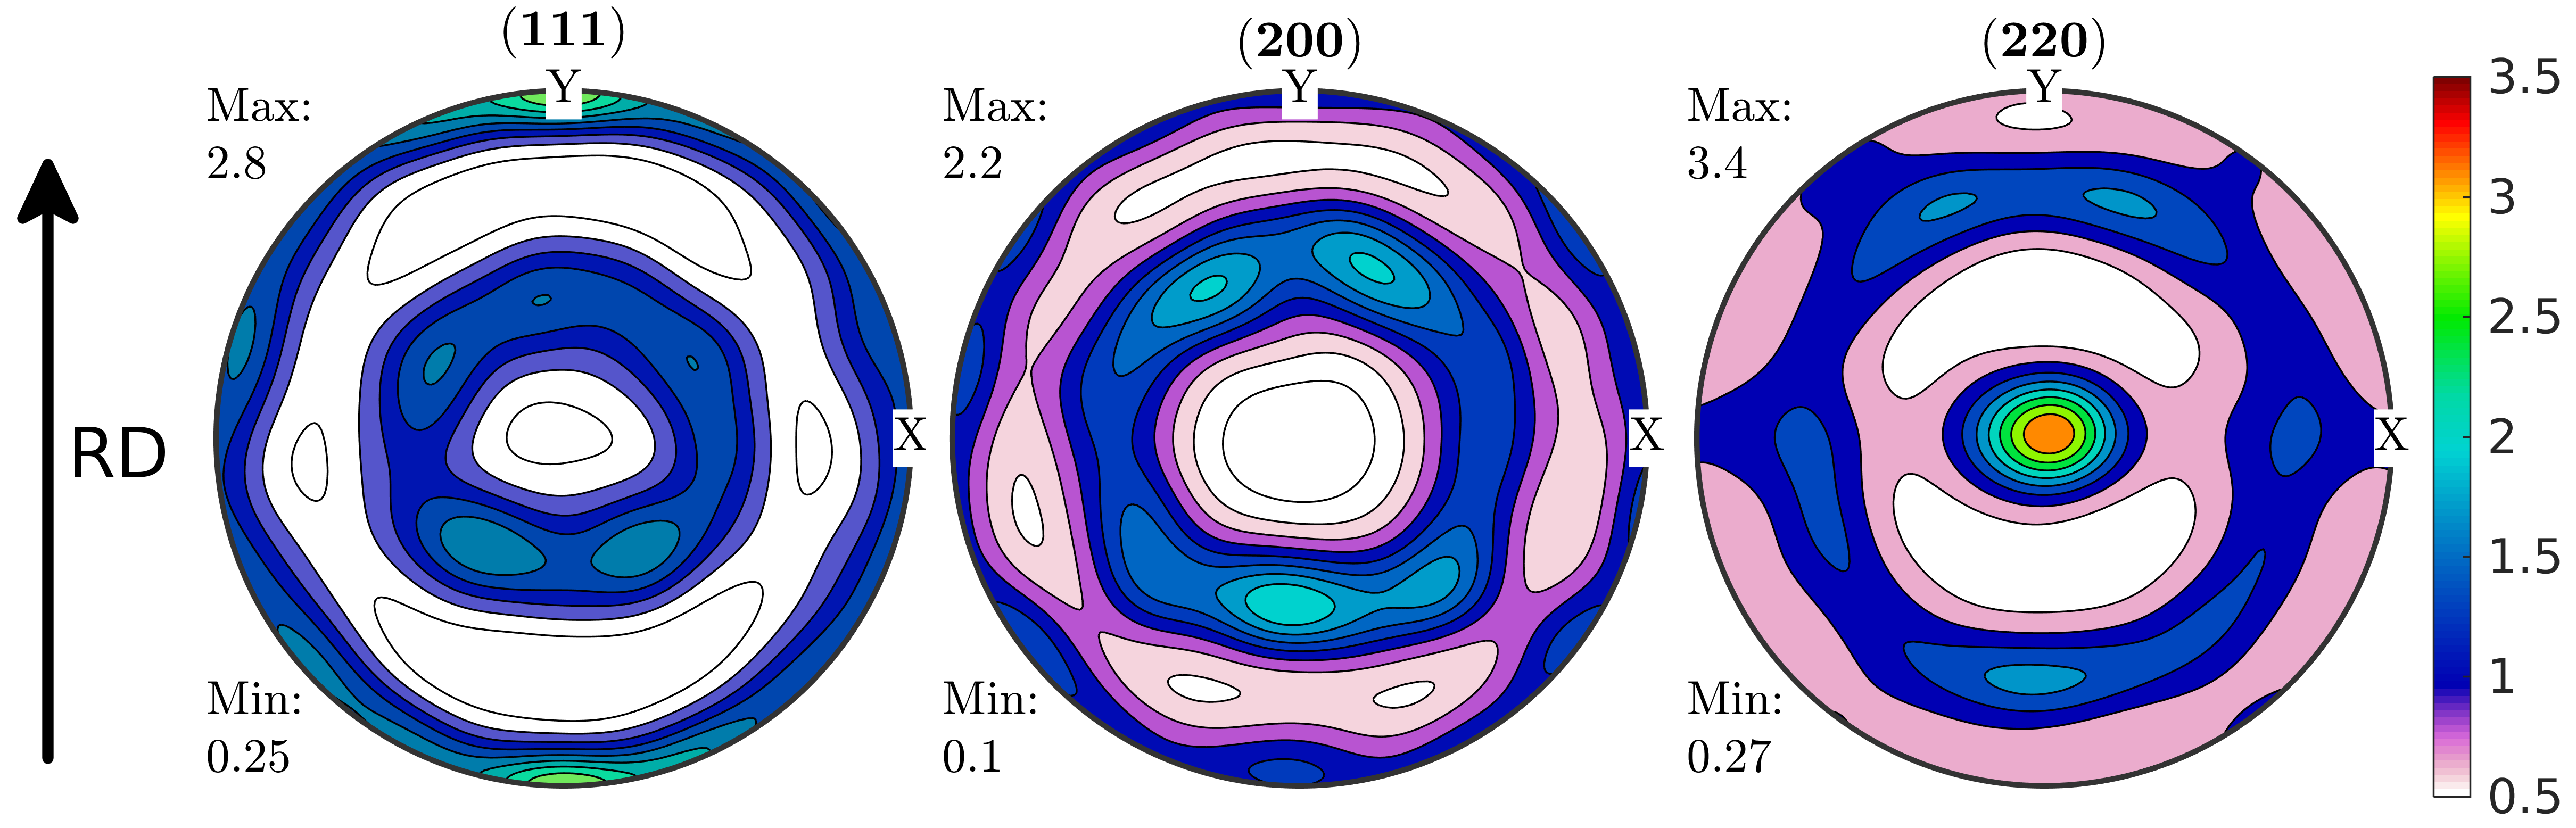
\includegraphics[width=\textwidth]{F138_Rec_RD}
  \caption{Figuras de Polos recalculadas para el acero F138 laminado. Puede apreciarse la presencia de la fibra \{110\}\textless uvw\textgreater, que suele verse en este material cuando es deformado por compresión. Esta anisotropía puede indicar de que el laminado ha introducido maclas en el material.}
  \label{fig:F138PF}
\end{figure}

Al observar la sección $\varphi_2 \ = \ 0$\,$^{\circ}$ de la FDO se aprecia que la fibra no tiene intensidad uniforme, sino que la misma incrementa su intensidad en la componente  G/B(T) (\{110\}\textless 111\textgreater). 
La componente Goss (\{110\}\textless 001\textgreater), que fue observada claramente al estudiar la textura empleando rayos X de laboratorio con geometría de reflexión, tiene aquí una intensidad similar a la del resto de la fibra.
Esta diferencia fue atribuida a heterogeneidades en la textura a lo largo de la dirección ND en el material laminado, apreciables en los experimentos de transmisión pero no en los de reflexión. 
Dado que en los experimentos de difracción se obtiene la información de todo el volumen del material, la textura resultante es el promedio de las heterogeneidades presentes en el mismo, por lo que experimentos en los que se promedian volúmenes distintos pueden dar resultados ligeramente diferentes.
En este caso, las mediciones de textura realizadas con rayos X de laboratorio emplean una geometría de reflexión, por lo que toda la información obtenida proviene de los cristales que se encuentran en la superficie del material.
La mediciones realizadas en sincrotrón, por otro lado, emplean una geometría de reflexión, por lo que la información de la superficie se superpone con la que se encuentra en el interior del mismo.
Como la textura en el interior del material laminado no es exactamente igual a la de la superficie, y como dicha heterogeneidad existe a lo largo de la dirección ND, la intensidad de las FP y de las FDO obtenidas de las mediciones de sincrotrón se verán ``suavizadas'' respecto de aquellas que fueron obtenidas empleando una geometría de reflexión en la superficie del material.

\begin{figure}[!htb]
  \centering
  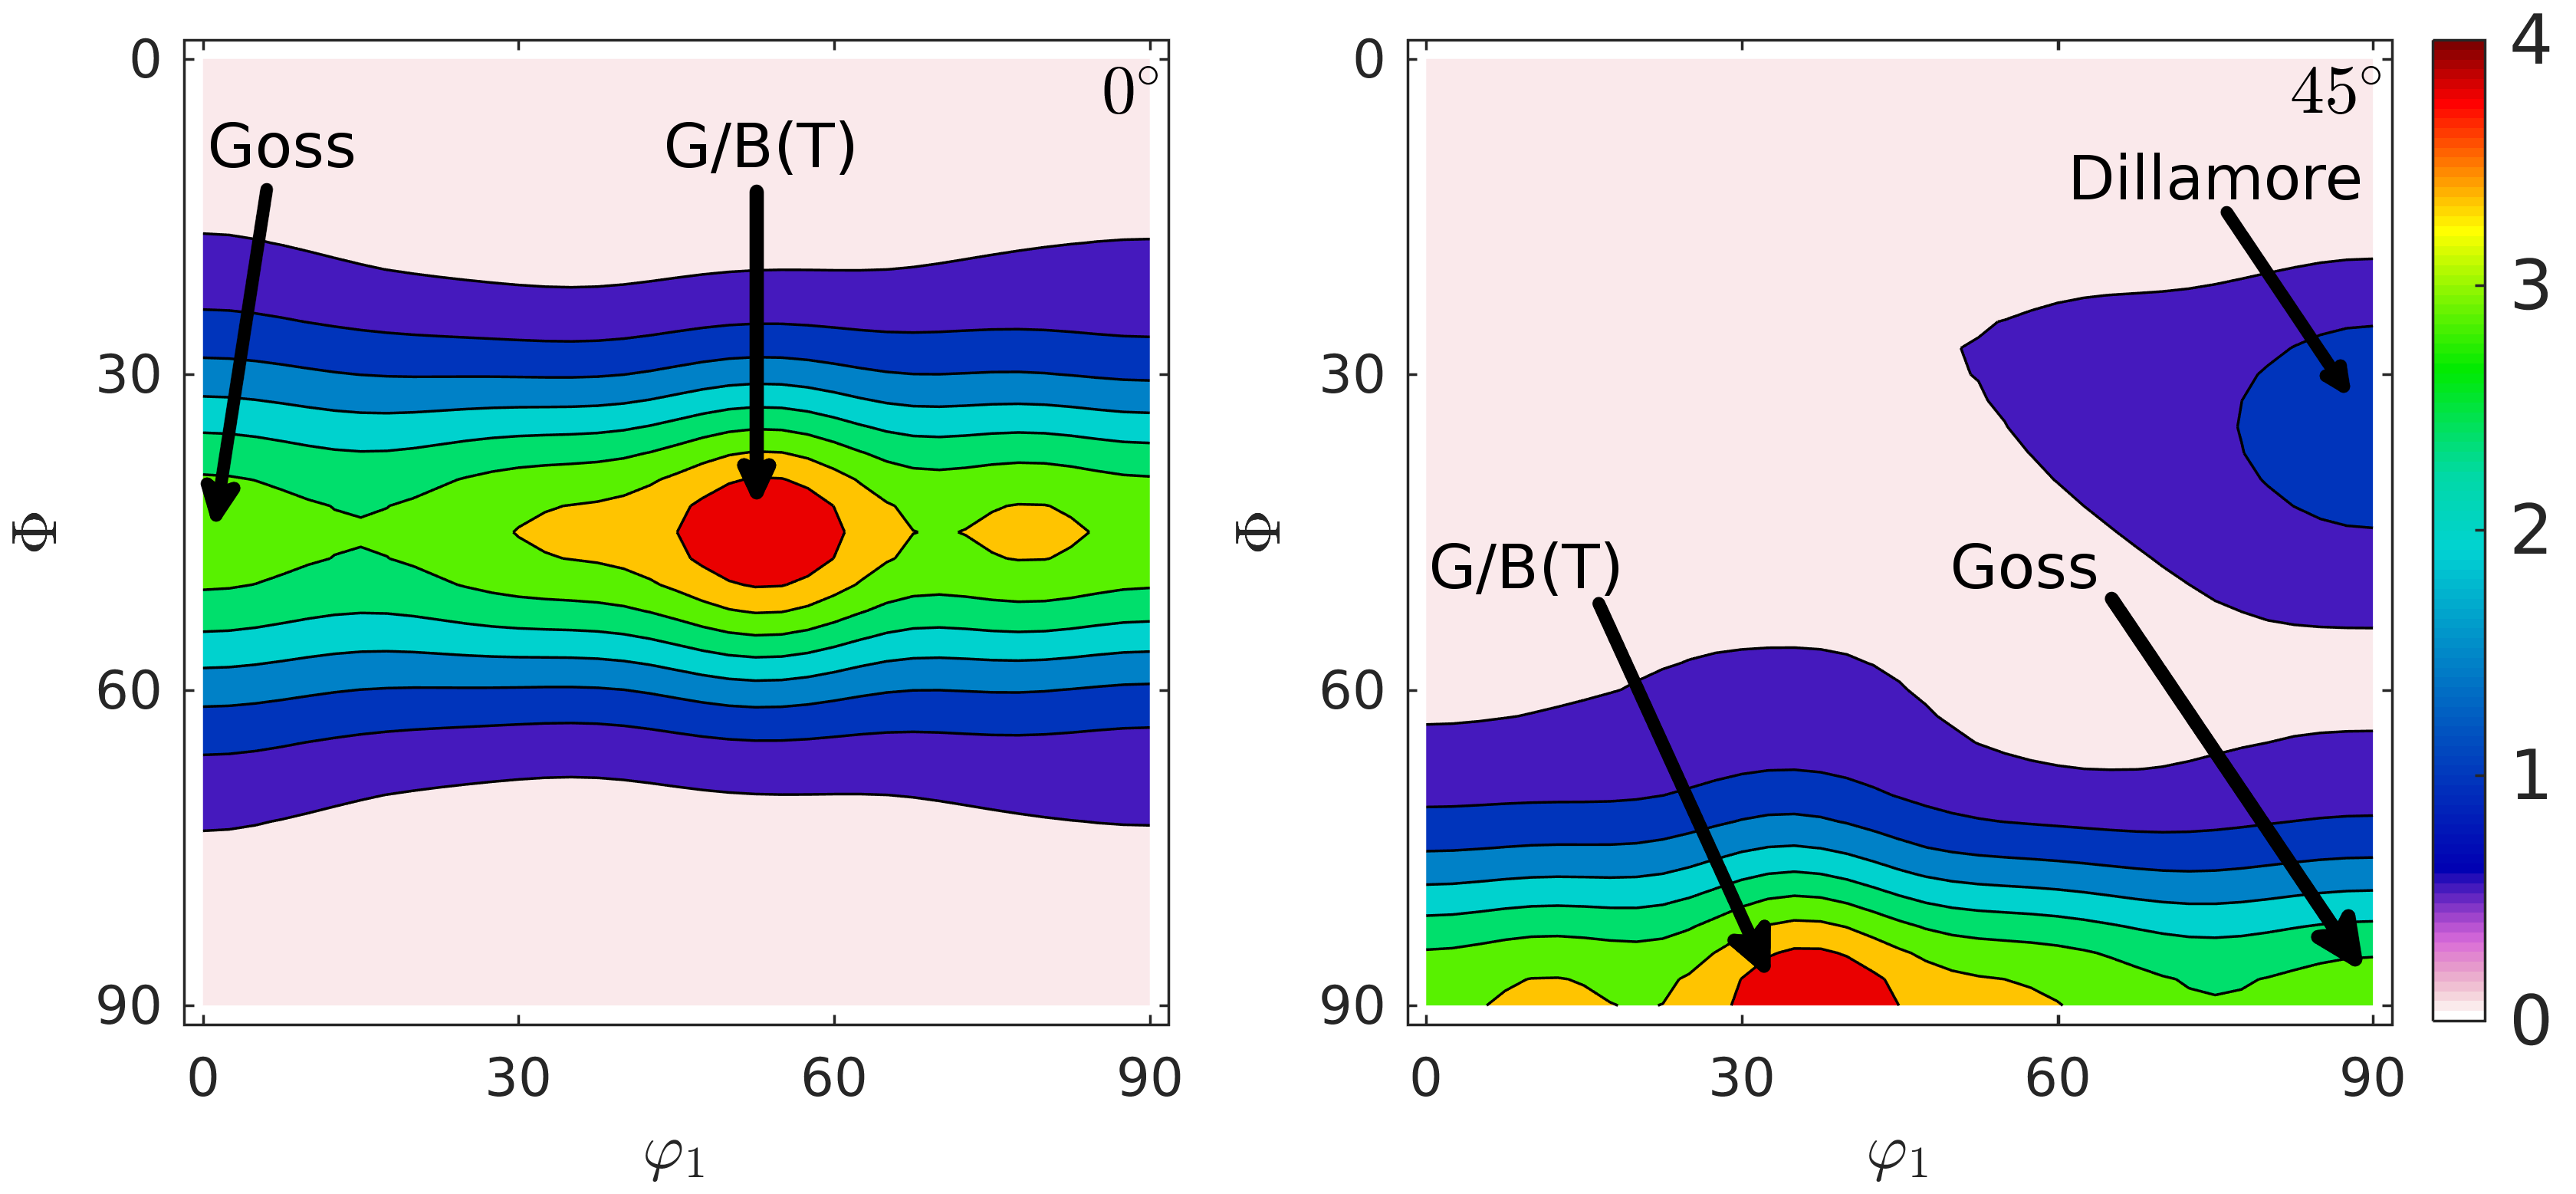
\includegraphics[width=\textwidth]{F138_odf_Arrow}
  \caption{Secciones $\varphi_2 \ = \ 0$\,$^{\circ}$ y $\varphi_2 \ = \ 45$\,$^{\circ}$ de la FDO del acero F138 laminado. La fibra \{110\}\textless uvw\textgreater también puede verse en la sección $\varphi_2 \ = \ 0$\,$^{\circ}$, donde también puede verse que dicha fibra tiene un máximo en la componente G/B(T). La sección $\varphi_2 \ = \ 45$\,$^{\circ}$ muestra la misma fibra que se ve en la sección $\varphi_2 \ = \ 0$\,$^{\circ}$, pero además puede apreciarse la presencia de la componente Dillamore en las coordenadas $(\varphi_1, \Phi, \varphi_2) \ = \ (90, 30, 45)$\,$^{\circ}$.}
  \label{fig:F138ODF}
\end{figure}

La sección $\varphi_2 \ = \ 45$\,$^{\circ}$ muestra las mismas componentes observadas en la sección $\varphi_2 \ = \ 0$\,$^{\circ}$, aunque aquí puede apreciarse la presencia de la componente Dillamore en las coordenadas $(\varphi_1, \Phi, \varphi_2) \ = \ (90, 30, 45)$\,$^{\circ}$.

La textura que se muestra en las FDO de la Fig. \ref{fig:F138ODF} es esperable para materiales FCC laminados, aunque también se nota una fuerte anisotropía del material en la dirección cristalina \{220\}, que se asocia a la baja energía de falla de apilamiento en aceros\cite{Sathiaraj2015,Saleh2012}, aunque los análisis realizados empleando el método CMWP en distintas direcciones indicaron que el laminado de 70\,\% fue poco efectivo en introducir maclas, sobre todo cuando se comparón con la cantidad introducida al deformar la muestra por ECAE.
Para tener como referencia, las estimaciones de CMWP indicaron que la proporción de maclas se encontraba por debajo de las 3 fallas de apilamiento/$\mu$m, lo cual sugiere además que la contribución de las fallas de apilamiento al ensanchamiento de los picos de difracción puede dejarse de lado.
Esto último es particularmente importante teniendo en cuenta que en la próxima sección se estudiará en ensanchamiento de los picos de difracción empleando el método de Langford, ya que como se explicó en la Sec. \ref{SS:Twin} la contribución de las fallas de apilamiento no se puede introducir sencillamente en dicho modelo.

Los estudios realizados aplicando los métodos CMWP y Williamson-Hall revelaron tamaños de dominio del orden de los 50 nm para las tres direcciones de muestra, con valores algo mayores para los tamaños de dominios observados en la dirección de laminado, RD.
La densidad de dislocaciones obtenida fue del orden de 1\,$\times$\,10$^{16}$\,m$^{-2}$ para las direcciones RD y TD, y del orden de 1.5\,$\times$\,10$^{16}$\,m$^{-2}$ para la dirección ND.
Esta discrepancia recuerda los discutido en el Cap. \ref{C:IF}, donde se mencionó que la densidad de dislocaciones debe ser una cantidad independiente de la dirección de la muestra que se esté observando.

Dado que tanto CMWP como Williamson-Hall hacen uso del modelo del factor de contraste, ambos consideran que toda anisotropía se debe a la mayor o menor visibilidad de las dislocaciones en una dada dirección, por lo que es de suponer que si se observa una dependencia de la densidad de dislocaciones con la dirección de la muestra, es porque o bien los factores de contraste no fueron empleados correctamente o bien porque existe cierta anisotropía en alguna población cristalina que no puede explicarse por efectos geométricos.

Para determinar cuál es la situación para el acero F138, los autores de \cite{Devincentis2017} aplicaron un método un tanto diferente al empleado en el Cap. \ref{C:IF}, que consistió en observar las curvas de Williamson-Hall para detectar si alguna de las familias de planos presentaba alguna anomalía que no se pudiera justificar a partir del cálculo de los factores de contraste.
Parte de los resultados se observan en las gráficas de la Fig. \ref{fig:F138NatiWHvsEquipos}, que muestran las curvas de Williamson-Hall obtenidas a partir de las mediciones realizadas con un difractómetro X'Pert de laboratorio (a)  y las realizadas en DESY (b), después de corregir los anchos de pico por el efecto de los factores de contraste.

\begin{figure}[!htb]
  \centering
  \includegraphics[width=\textwidth]{F138_WH_Equipos}
  \caption{Curvas de Williamson-Hall Modificado para el acero F138 laminado y recocido a diferentes temperaturas. (a) A partir de rayos X de laboratorio (b) A partir de rayos X de sincrotrón. Puede verse que para la muestra laminada, el pico \{220\} se aparta de la curva definida por el ensanchamiento del resto de los picos, mientras que el comportamiento anómalo desaparece al recocer el material. Gráficas obtenidas de \cite{Devincentis2017}.}
  \label{fig:F138NatiWHvsEquipos}
\end{figure}

Como ya se discutió en el Cap. \ref{C:Intro}, el efecto de los factores de contraste en las gráficas de Williamson-Hall es el de corregir las discontinuidades observadas a causa del ensanchamiento anisotrópico, haciendo que los anchos medidos dibujen una curva suave y monótona al ser graficados en función de $\sin{\theta_B}*\sqrt{C_{av}}$.
En ese sentido, se observa que para las muestras laminadas y recocidas la corrección por factor de contraste es efectiva, ya que todos los picos medidos caen sobre la misma curva, sin embargo, para la muestra laminada, que denominaremos F138R70, se tiene una dispersión mayor en la gráfica de Williamson-Hall .
En este caso puede apreciarse que el ensanchamiento anómalo se presenta en los planos que tienen su dirección \{220\} en la dirección ND.
Dicho comportamiento consiste en que el ancho del pico \{220\}, después de ser corregido por el efecto de su respectivo factor de contraste, se encuentra claramente alejado de la curva definida por los ensanchamientos obtenidos del resto de los picos.

Resulta notable el hecho de que la anomalía desaparece luego de recocer la muestra y que la misma se observa independientemente del equipo que se emplea para determinar el ancho de los picos, lo que hace improbable que el efecto observado se deba a un artefacto instrumental creado por el mismo equipo.
Es más, también se observó que este apartamiento existe sólo en los difractogramas medidos a lo largo de ND, mientras que las curvas de Williamson-Hall medidas a lo largo de RD y TD son suaves y monótonas.

Lo primero que se hizo para determinar el origen de la anomalía fue estudiar el efecto de la textura en en los factores de contraste obtenidos para las muestras laminadas, cuyos valores pueden apreciarse en la Fig. \ref{fig:F138NatiContrast}.
Puede verse que los factores de contraste obtenidos para las tres direcciones son relativamente similares, aunque se observa una dispersión levemente mayor para los planos \{220\}, en particular en la dirección ND, lo cual sugiere una conclusión similar a la obtenida en el Cap. \ref{C:IF}, es decir, que la anisotropía en la acumulación de defectos que no puede ser explicada completamente a partir del modelo del factor de contraste, lo que implicaría que distintas poblaciones cristalinas han desarrollado microestructuras diferentes.

\begin{figure}[!htb]
  \centering
  \includegraphics[width=0.6\textwidth]{F138_WH_DESY_Contrast}
  \caption{Factores de contraste para las tres direcciones con los anchos medidos en DESY. Sacado de \cite{Devincentis2017}.}
  \label{fig:F138NatiContrast}
\end{figure}

Si el menor ensanchamiento de los picos 220 de la dirección ND no se puede explicar a partir del valor de los factores de contraste, queda evaluar la posibilidad de que que los cristales orientados según la dirección \textless220\textgreater$\parallel$ND exhiban un ensanchamiento inferior al resto de las componentes de textura del material, debido a que han acumulado una cantidad de defectos notablemente menor que el resto de las componentes.
En este sentido, las dos situaciones más probables implican que los cristales con dirección \textless220\textgreater$\parallel$ND tienen dominios más grandes y/o han acumulado menos dislocaciones, ya que en ningún caso se observa variación en la capacidad de acumular maclas, que es el tercer tipo de defecto que es razonable buscar en este tipo de acero.

El estudio de esta posibilidad se realizó empleando microscopía electrónica de barrido, por medio de la técnica de EBSD.
En particular, dado que la textura está marcada por presencia de la fibra \{110\}\textless uvw\textgreater, y que la mayor anisotropía se observó en los planos \{220\}, se realizó un estudio similar al descripto en el Cap. \ref{C:IF}, realizando particiones seleccionando cristales en función de la orientación de sus planos \{110\}, y comparando la estructura de defectos de las diferentes poblaciones. 

En la Fig. \ref{fig:F138EBSDNati} se aprecian dos de los principales resultados de este estudio, el tamaño de grano para distintas direcciones de muestra (Fig. \ref{fig:F138EBSDNati}-a) y la distribución de GNDs (Fig. \ref{fig:F138EBSDNati}-b), para las diferentes particiones de interés, definidas en función de la orientación de la familia de planos \{220\} respecto de los ejes principales de la muestra.

\begin{figure}[!htb]
  \centering
  \includegraphics[width=\textwidth]{F138_EBSD_SizeyGNDvsDirection}
  \caption{Tamaño de dominio (longitud de intercepción) y GND según dirección cristalina. Imágenes obtenidas de \cite{Devincentis2017}.}
  \label{fig:F138EBSDNati}
\end{figure}

Los resultados de EBSD son consistentes con lo observado a través de los experimentos de XRD, ya que el tamaño de grano de los cristales con dirección \textless220\textgreater$\parallel$ND es notablemente mayor que la de los cristales de la partición complementaria, mientras que no se observa un cambio tan importante cuando se observa a la muestra en las direcciones TD y RD.
Adicionalmente, según lo mostrado en la distribución de GND de la Fig. \ref{fig:F138EBSDNati}-b, los cristales con orientación \textless220\textgreater$\parallel$ND tienen en promedio menos dislocaciones que los que no se encuentran con la dirección \{220\} paralela a ND.
Vale la pena notar que la densidad de dislocaciones medida por EBSD da un valor que es aproximadamente dos órdenes de magnitud inferior a lo estimado por medio de Williamson-Hall y CMWP.
Esto probablemente se deba a la presencia de dislocaciones en arreglos compactos, las cuales son en general invisibles a la técnica de EBSD, además de dislocaciones que generan misorientaciones de muy bajo ángulo. 
Esto se debe a que el haz de rayos X generado en el sincrotrón posee una brilliancia (intensidad sobre divergencia angular) mucho más elevada que el haz de electrones de un microscopio electrónico, más detectables por medio de la técnica de difracción de rayos X que por EBSD, debido a la elevada brilliancia de la radiación sincrotrón.

Las mediciones de EBSD también revelaron que la partición \textless220\textgreater$\nparallel$ND posee, a diferencia del resto de las particiones analizadas, una proporción importante de \textit{bordes de grano de alto ángulo} (HAGB, por sus siglas en inglés), lo que sugiere que el laminado produjo recristalización dinámica en el material.
El hecho de que la recristalización haya ocurrido en una población cristalina particular sugiere a su vez que distintas poblaciones de cristales han acumulado una cantidad de energía muy diferente como consecuencia del laminado, lo que contribuye aún más a la idea de la orientación de los cristales es un factor importante a la hora de determinar la capacidad de un material de acumular defectos.
En \cite{Devincentis2015} lo autores observaron un comportamiento similar sobre el mismo material, aunque esta vez al ser sometido a 4 pasadas de ECAE.

Los HAGB se caracterizan por ser arreglos compactos con alta densidad de dislocaciones, en contraposición con los \textit{bordes de grano de bajo ángulo} (LAGB, por sus siglas en inglés), que tienden a acumular menos dislocaciones que además se encuentran menos correlacionadas.
En este sentido, es razonable esperar que los cristales cuyos planos \{220\} son paralelos a ND revelen menor número de dislocaciones que aquellos de la partición complementaria, y por lo tanto menor ensanchamiento, que aquellos cristales que no tengan ésta característica.

\nomenclature{HAGB}{Siglas en inglés para Bordes de grano de alto ángulo (High Angle Grain Boundary).}
\nomenclature{LAGB}{Siglas en inglés para Bordes de grano de bajo ángulo (Low Angle Grain Boundary).}
\newpage
\section{Estudio de la microestructura por el método de Langford y figuras de polos generalizadas}\label{S:F138LANG}
En la Fig. \ref{fig:F138ODFComp}-a se encuentra repetida la FDO que se mostró en la Fig. \ref{fig:F138ODF}, sólo que ahora se encuentra acompañada por las FDOG de tamaño de cristalita y densidad de dislocaciones, Figs. \ref{fig:F138ODFComp}-b y \ref{fig:F138ODFComp}-c, respectivamente.
El comportamiento observado en este caso guarda reminiscencias a lo observado en el Cap. \ref{C:IF} para acero libre de intersticiales, donde las componentes favorecidas por la textura tienen mayor tamaño de cristalita y acumulan menos dislocaciones.

\begin{figure}[!htb]
    \centering
    \begin{subfigure}[!htb]{0.965\textwidth}
        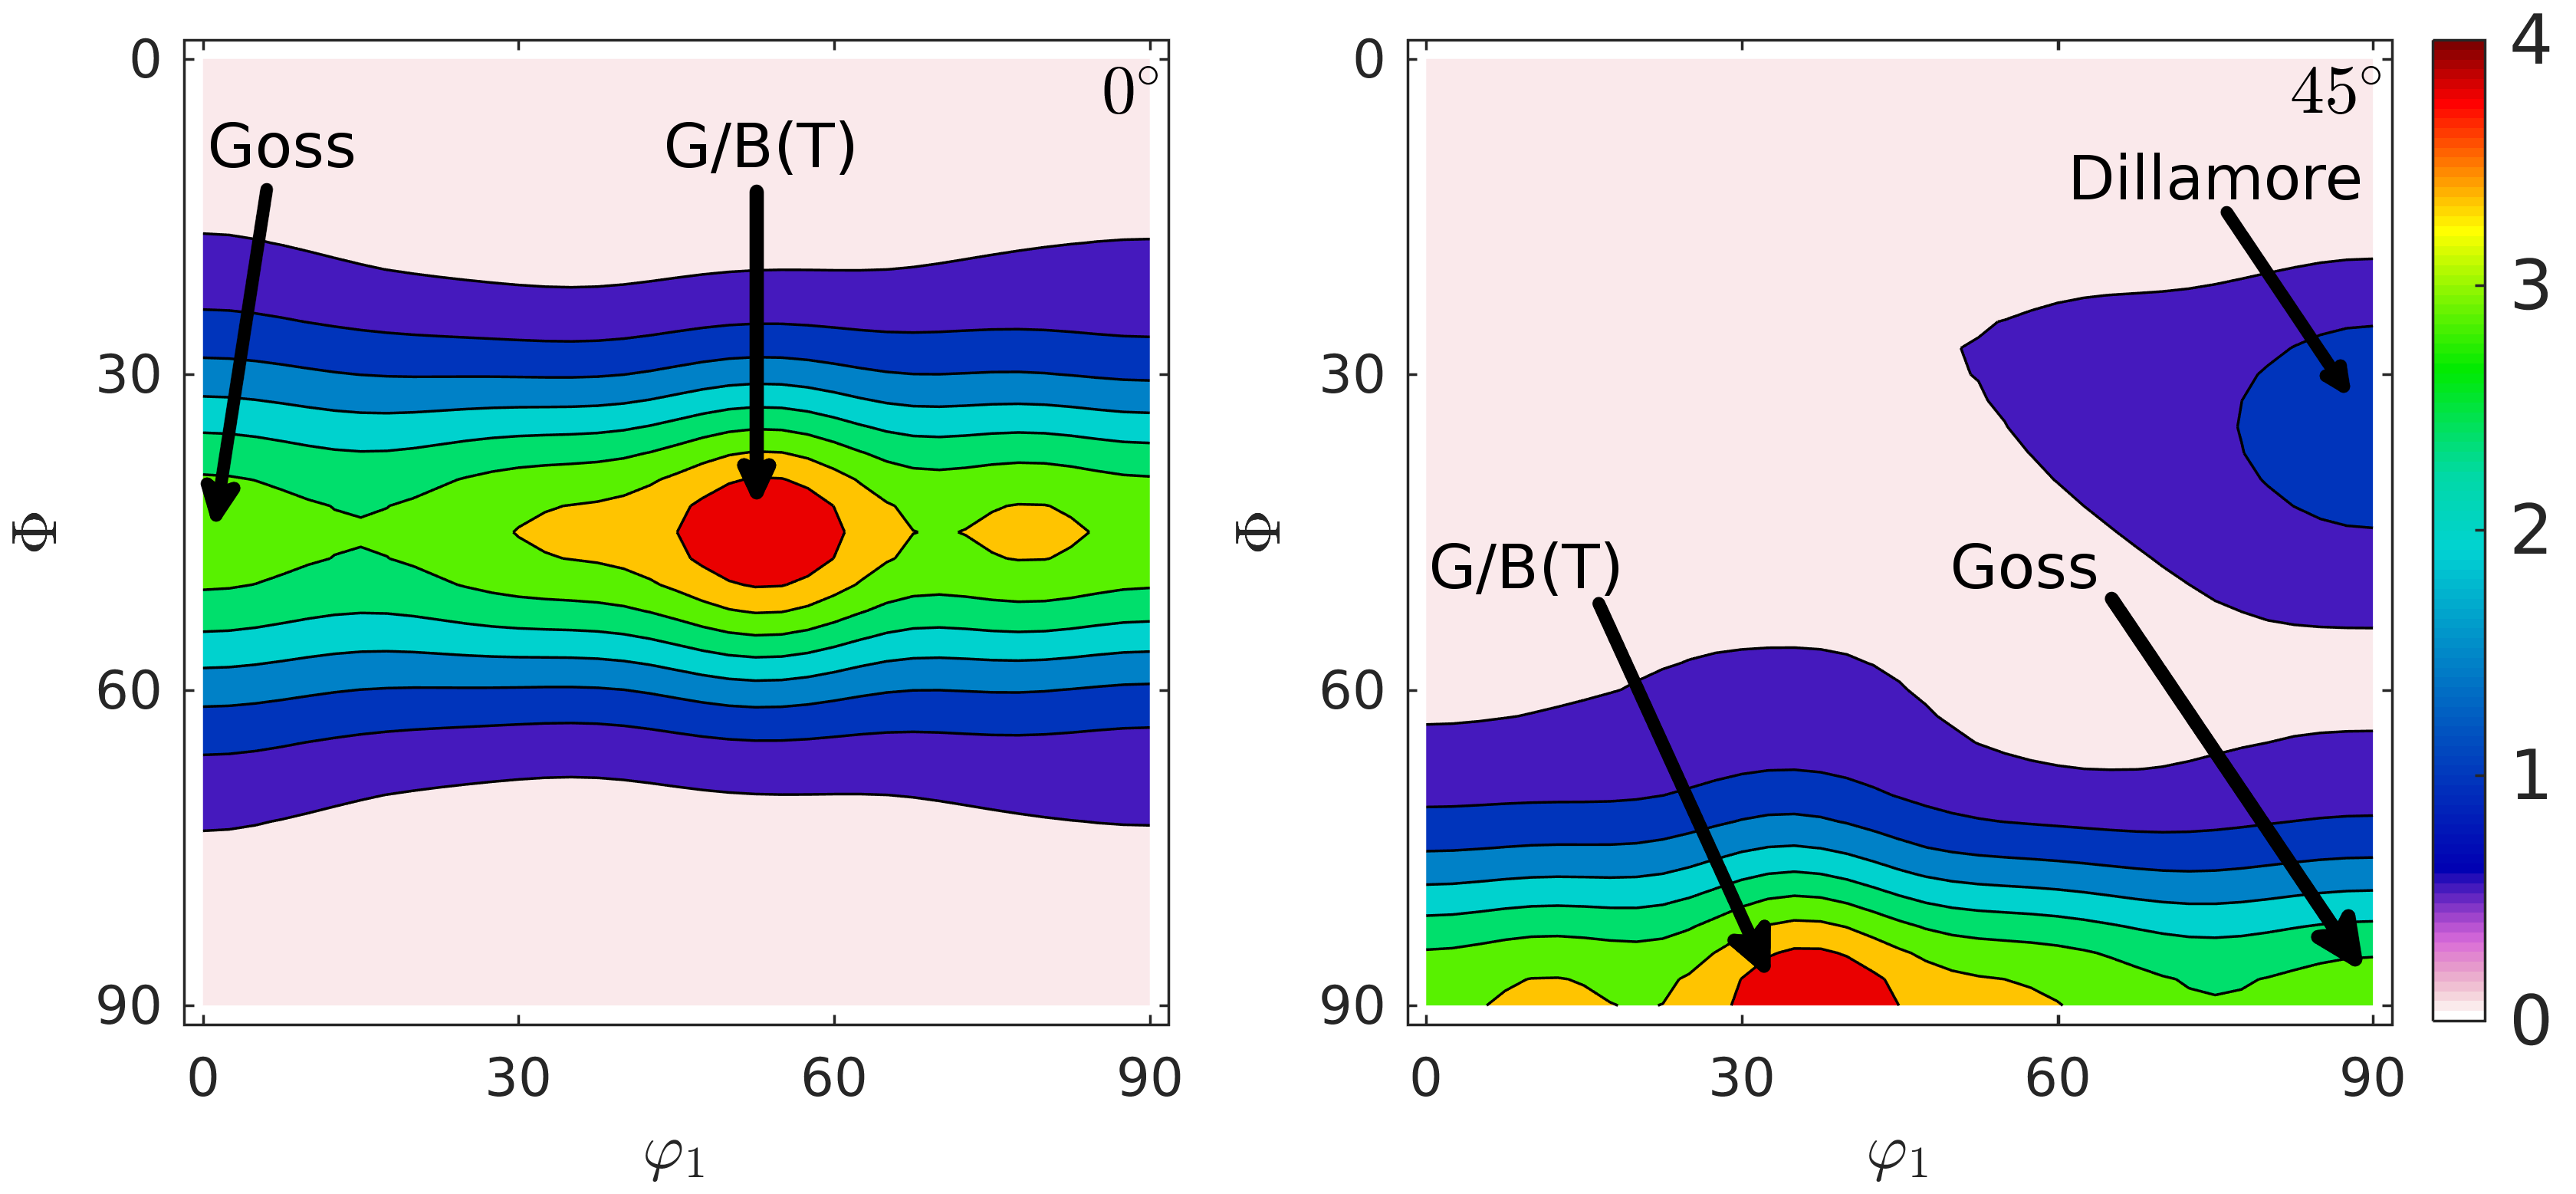
\includegraphics[width=0.965\textwidth]{F138_odf_Arrow}
        \caption{}
        \label{fig:F138ODFCompODF}
    \end{subfigure}
   \\ 
    \begin{subfigure}[!htb]{\textwidth}
        \includegraphics[width=\textwidth]{F138_Sizeodf}
        \caption{}
        \label{fig:F138ODFCompSizeODF}
    \end{subfigure}
   \\ 
    \begin{subfigure}[!htb]{\textwidth}
        \includegraphics[width=\textwidth]{F138_Strainodf}
        \caption{}
        \label{fig:F138ODFCompStrainODF}
    \end{subfigure}
    \caption{Comparación de las ODF. \ref{fig:F138ODFComp}-\subref{fig:F138ODFCompODF} FDO. \subref{fig:F138ODFCompSizeODF} FDOG de tamaño de cristalita. \subref{fig:F138ODFCompStrainODF} FDOG de dislocaciones.}
    \label{fig:F138ODFComp}
\end{figure}

Analizando las principales componentes de textura se puede observar que según el análisis de Langford la fibra \textless220\textgreater$\parallel$ND posee los tamaños de dominio más grandes, con los máximos yendo de la componente Goss a la G/B(T).
Puede apreciarse además que en esta fibra, la intensidad de la textura correlaciona muy bien con el tamaño de cristalita a lo largo de toda la fibra.
En el caso de las componentes que poseen una intensidad baja en la FDO, la FDOG de cristalita muestra un tamaño intermedio, similar incluso a la de los cristales con población del orden de 1 m.r.d., e.g. la componente Dillamore.

La situación es bastante diferente cuando se compara la FDOG de densidad de dislocaciones con la textura.
En este caso, las zonas más cargadas de dislocaciones son las vecinas a la fibra \textless220\textgreater$\parallel$ND, observándose los máximos en las regiones más desfavorecidas por la textura.
La única población favorecida por la textura que ha acumulado dislocaciones es la componente Goss, mientras que la componente G/B(T) posee una cantidad de dislocaciones próxima al mínimo. 
La componente Dillamore, por otro lado posee una cantidad de dislocaciones intermedia, comparable a la observada en las orientaciones más desfavorecidas por la textura, similarmente a lo observado en la FDOG de tamaño de cristalita.

Como para este material se observó una anisotropía bien marcada en la dirección ND, parece últi observar también las figuras de polos inversas, así como su contraparte generalizada para tamaño de dominio y densidad de dislocaciones.

\begin{figure}[!htb]
  \centering
  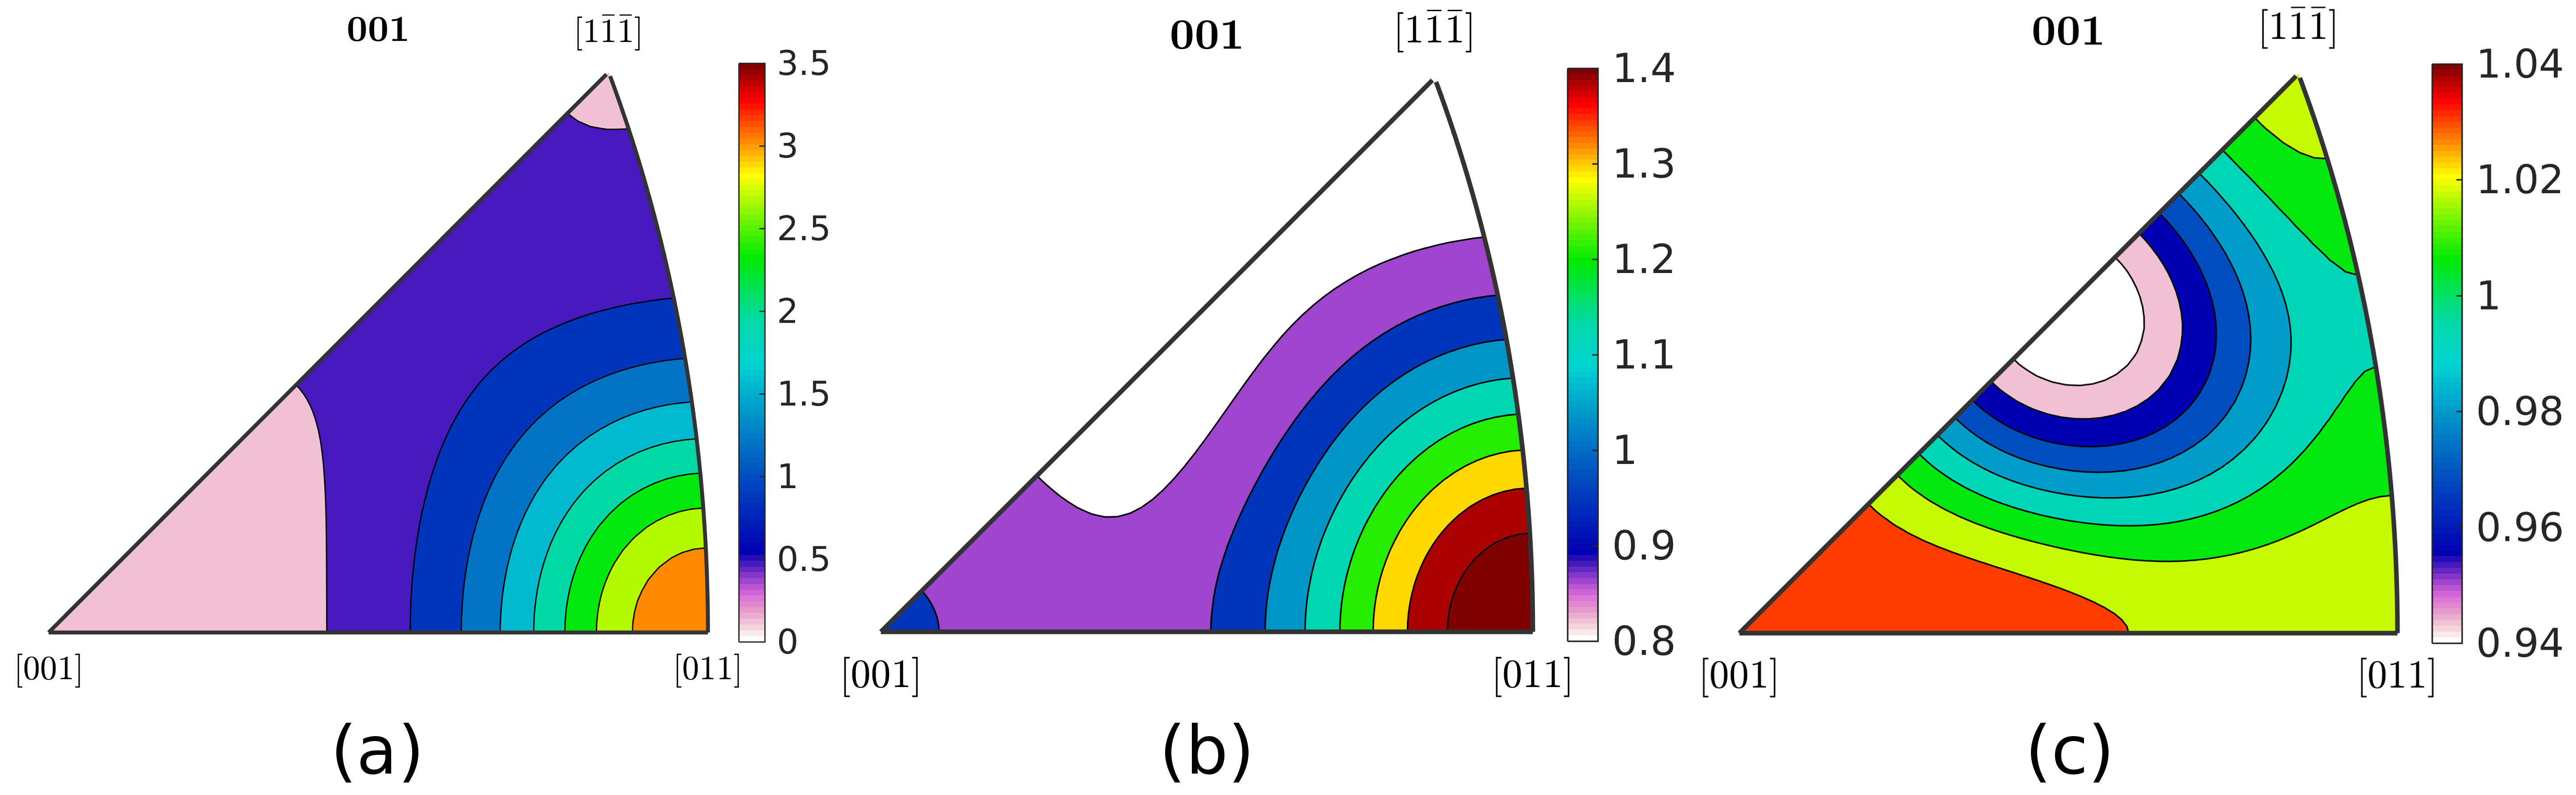
\includegraphics[width=\textwidth]{F138_zipdfcomp}
  \caption{Comparacion de las IPDF. (a) IPDF. (b) IPDFG De tamaño de cristalita. (c) IPDFG de dislocaciones.}
  \label{fig:F138IPDFComp}
\end{figure}

\nomenclature{m.r.d.}{Multiples of Random Distribution, Múltiplos de la Distribución Aleatoria.}
\newpage
\section{Discusión de resultados}\label{S:F138Dis}
Explicar algo de por qu las poblaciones vacías tienen dominios mas grandes que las random.

\newpage
\section{Conclusiones}\label{S:F138Conclusiones}
